\chapter{Operational Semantics}
In this chapter some of the operational semantics of NISSE will be shown. In order to be able to read the operational semantics a few things should be known. \\
\texttt{S} denotes slides and is an environment consisting of variables (slides) pointing to a location with the \texttt{body} of the slide. \\
Also included in the environment is the keyword \texttt{next} which points to the next empty variable, and the function \texttt{new} which gets the next variable after its parameter. \\
\texttt{env} denotes an environment for settings, which also consists of variables pointing to locations containing the value of that setting. \texttt{env} does not need the \texttt{next} keyword and the \texttt{new} function because all of the settings is predefined and the only thing changed is the settings' value.
\\ \\
\noindent{$[slideshow]$}
\[ \langle S, env \rangle \ra show \]
The transition describes how the entire slideshow is made, which are with elements in \texttt{S} that has the variables in the environment.
\\ \\ 
\noindent{$[specification]$}
\[ \condinfrule{\langle slide, S \rangle \ra S' \langle setting, env \rangle \ra env'} { \langle slide~setting, S, env \rangle \ra S', env'}{} \]
This transition describes when the command slide is executed in \texttt{S}, which changes S. And when a setting is executed in the variable environment, the environment is changed.
\\ \\
\noindent{$[setting]$}
\[ \condinfrule{\langle shortident, env \rangle \ra env' \langle scope \rangle} { \langle @ setting \{ shortident | scope \}, env \rangle \ra env'}{} \]
This transition describes the inside of a setting, how the element inside a setting block changes in the variable environment in the specific scope.
\\ \\
\noindent{$[slide]$}
\[ \condinfrule{\langle block, S[L \mapsto block] [next \mapsto new L] \rangle \ra S'} { \langle block, S \rangle \ra S'}{} \]
\[ L = S(next)\]
This transition describes when a block is executed in \texttt{S}. This inserts the slide inside \texttt{S}, and moves the pointer to the next location where a slide can be inserted.
\\ \\
\noindent{$[block]$}
\[ \condinfrule{\langle setting, env \rangle \ra env' \langle plain,~S \rangle \ra S� \langle num \rangle \langle ilist \rangle} { \langle begin~setting~plain~num~ilist~end, S \rangle \ra S'}{} \]
This transition shows how commands inside a block (slide) is executed, resulting in a change in a slide.
\\ \\
\noindent{$[plain]$}
\[ \condinfrule{\langle plaintext,~S \rangle \ra S� \langle shortblock,~env \rangle \ra env'} { \langle plaintext~shortblock,~S \rangle \ra S� }{} \]
This transition illustrates how plain text and/or shortblock is evaluated, with the environment \texttt{env}.
\\ \\
\noindent{$[shortblock]$}
\[ \condinfrule{\langle formatkwd \rangle \langle shortident, env \rangle \ra env' \langle plain \rangle} { \langle formatkwd \{shortident | plain\}, env \rangle \ra env'}{} \]
This transition changes the environment according to the \texttt{formatkwd} and \texttt{shortident}, for the specific plain text.
\\ \\
\noindent{$[shortident]$}
\[ \condinfrule{\langle env [L \mapsto V] \rangle \ra env'} { \langle kwd : V, env \rangle \ra env'}{} \]
\[ L = env(kwd)\]
This transition changes the environment according to the keyword and the variable \texttt{V}.


\subsection{Derivation Tree}
An example of a derivation tree is made in figure \ref{fig:DerivationTree} of the language code in listing \ref{lst:DerivationTree}.

\begin{lstlisting}[frame=single, caption=NISSE example, label=lst:DerivationTree]
@begin{slide}
    @title{Next lecture}(1)
    @subtitle{On 15.05.2012}(2)
    This was all for now.(3)
    Have a nice day.(4) 
    The current slideshow can be found at(5) @apply{@url:http://www.somelink.com | this link }(6).
@end{slide}
\end{lstlisting}

\noindent{The number at the end of almost each line i listing \ref{lst:DerivationTree} corresponds to the number in figure \ref{fig:DerivationTree}, for what it represents.}
%\begin{figure}
%\label{fig:DerivationTree}
%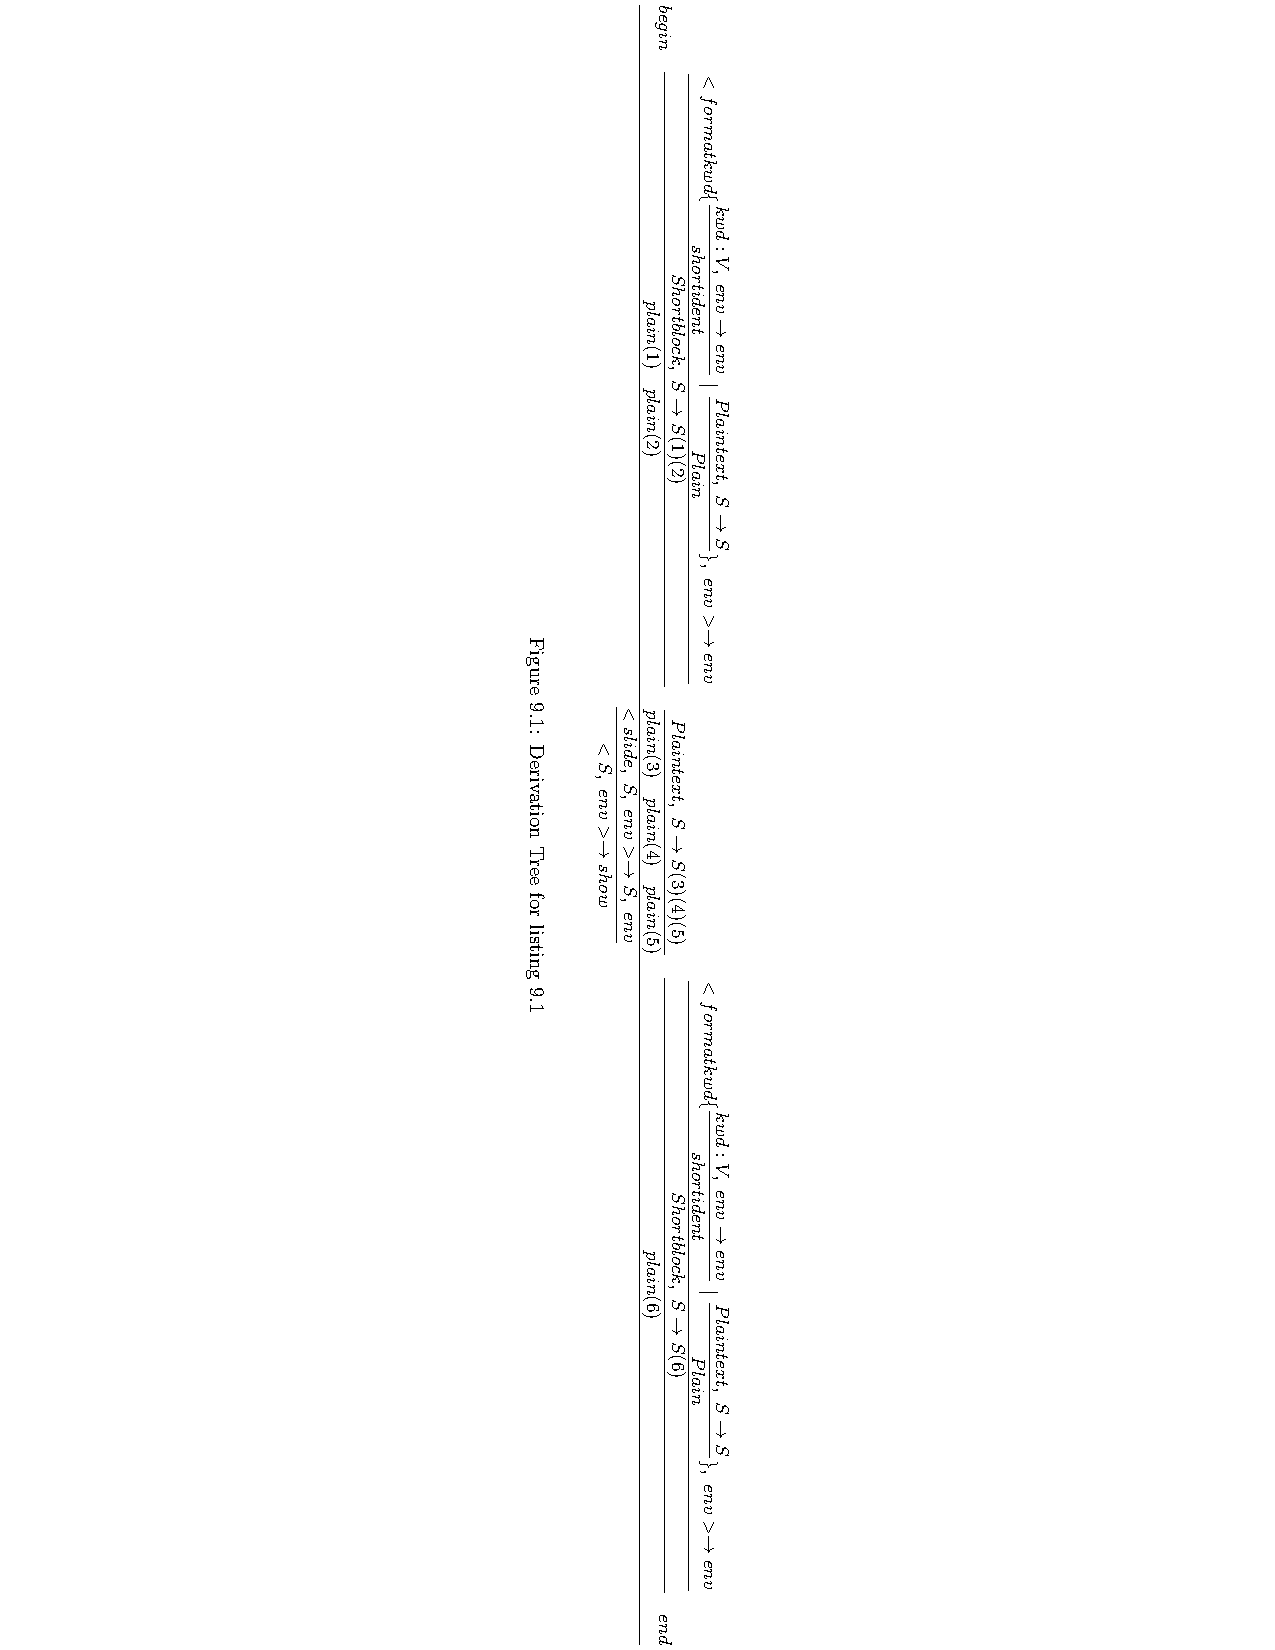
\includegraphics[scale=1]{images/derivation.pdf}
%\caption{Derivation Tree for listing \ref{lst:DerivationTree}}
%\end{figure}
\noindent{The \texttt{Shortblocks} in figure \ref{fig:DerivationTree} should be seen as being on the same line as \texttt{Plaintext}.
\texttt{plain(1)} and \texttt{plain(2)} in figure \ref{fig:DerivationTree} derives to two separate shortblocks. Even though the figure only shows one shortblock, which then changes the environment, according to the shortident and formatkwd, to the \texttt{Plain}, which derives to Plaintext, and changes the content of the slide. The same goes for \texttt{plain(6)}}

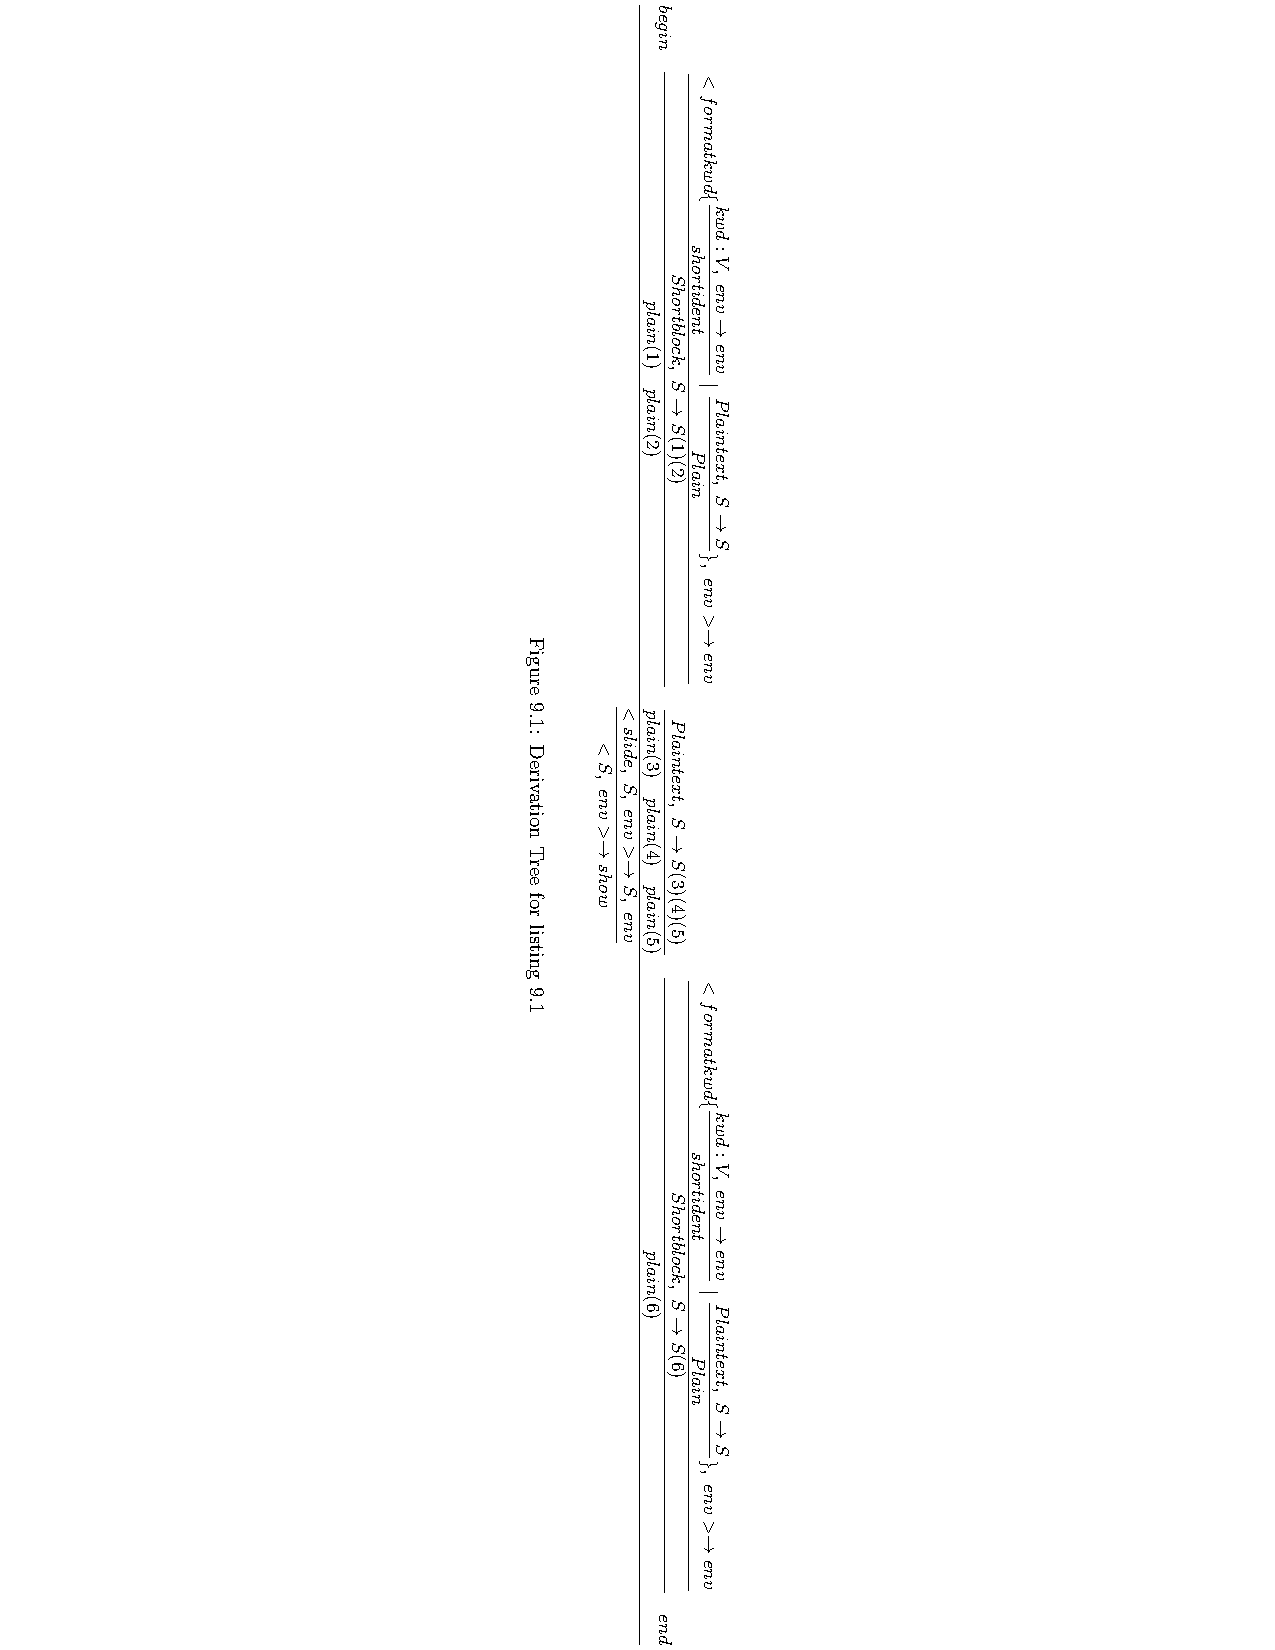
\includepdf{images/derivation}